\documentclass{article}
\usepackage[landscape]{geometry}
\usepackage{url}
\usepackage{multicol}
\usepackage{amsmath}
\usepackage{esint}
\usepackage{amsfonts}
\usepackage{tikz}
\usetikzlibrary{decorations.pathmorphing}
\usepackage{amssymb}
\usepackage[version=4]{mhchem}
\usepackage{graphicx}
\usepackage{float}
\usepackage{colortbl}
\usepackage{xcolor}
\usepackage{mathtools}
\usepackage{enumitem}
\usepackage[symbol]{footmisc}
\makeatletter

\newcommand*\bigcdot{\mathpalette\bigcdot@{.5}}
\newcommand*\bigcdot@[2]{\mathbin{\vcenter{\hbox{\scalebox{#2}{$\m@th#1\bullet$}}}}}
\renewcommand{\thempfootnote}{\fnsymbol{mpfootnote}}
\makeatother

\title{Unit 2 - Organic Chemistry}
\usepackage[T1]{fontenc}
\usepackage[utf8]{inputenc}
\usepackage[english]{babel}

\advance\topmargin-.8in
\advance\textheight3in
\advance\textwidth3in
\advance\oddsidemargin-1.5in
\advance\evensidemargin-1.5in
\parindent0pt
\parskip2pt
\newcommand{\hr}{\centerline{\rule{3.5in}{1pt}}}
%\colorbox[HTML]{e4e4e4}{\makebox[\textwidth-2\fboxsep][l]{texto}
\begin{document}

\begin{center}{\huge{\textbf{Unit 2 - Organic Chemistry}}}\\
\end{center}
\begin{multicols*}{3}

\tikzstyle{mybox} = [draw=black, fill=white, very thick,
    rectangle, rounded corners, inner sep=10pt, inner ysep=10pt]
\tikzstyle{fancytitle} =[fill=black, text=white, font=\bfseries]

%------------ Hybridization of Carbon ---------------
\begin{tikzpicture}
\node [mybox] (box){%
    \begin{minipage}{0.3\textwidth}
    \textbf{Bonding of Carbon}: a carbon atom has exactly half of a filled outer shell of electrons and an intermediate electronegativity, it can form covalent bonds with up to four other atoms.
    \begin{itemize}
        \item 4 single bonds
	\begin{itemize}
	    \item 4 identical $sp^{3}$ hybrid orbitals
	    \item 4 sigma bonds
	\end{itemize}
	\item 2 single bonds and 1 double bond
	\begin{itemize}
	    \item 3 identical $sp^{2}$ hybrid orbitals and 1 unchanged $p$ orbital
	    \item 3 sigma bonds and 1 pi bond
	\end{itemize}
	\item 1 single bond and 1 triple bond
	\begin{itemize}
	    \item 2 identical $sp$ hybrid orbitals and 2 unchanged $p$ orbitals
	    \item 2 sigma bonds and 2 pi bonds
	\end{itemize}
    \end{itemize}
    When a carbon atom is bonded to four different atoms, the resulting molecule has a \textit{tetrahedral} shape.
    \end{minipage}
};
%------------ Hybridization of Carbon Header ---------------------
\node[fancytitle, right=10pt] at (box.north west) {Hybridization of Carbon};
\end{tikzpicture}

%------------ Drawing Organic Molecules ---------------
\begin{tikzpicture}
\node [mybox] (box){%
    \begin{minipage}{0.3\textwidth}
    \begin{enumerate}
        \item condensed structural diagrams - does not show the carbon-hydrogen bonds; they are assumed to be present
	\item skeleton diagrams - each end of a straight line represents a carbon atom (unless otherwise specified) and each carbon is assumed to have as many hydrogen atoms bonded to it as is necessary to give it four bonds
    \begin{figure}[H]
        \centering
        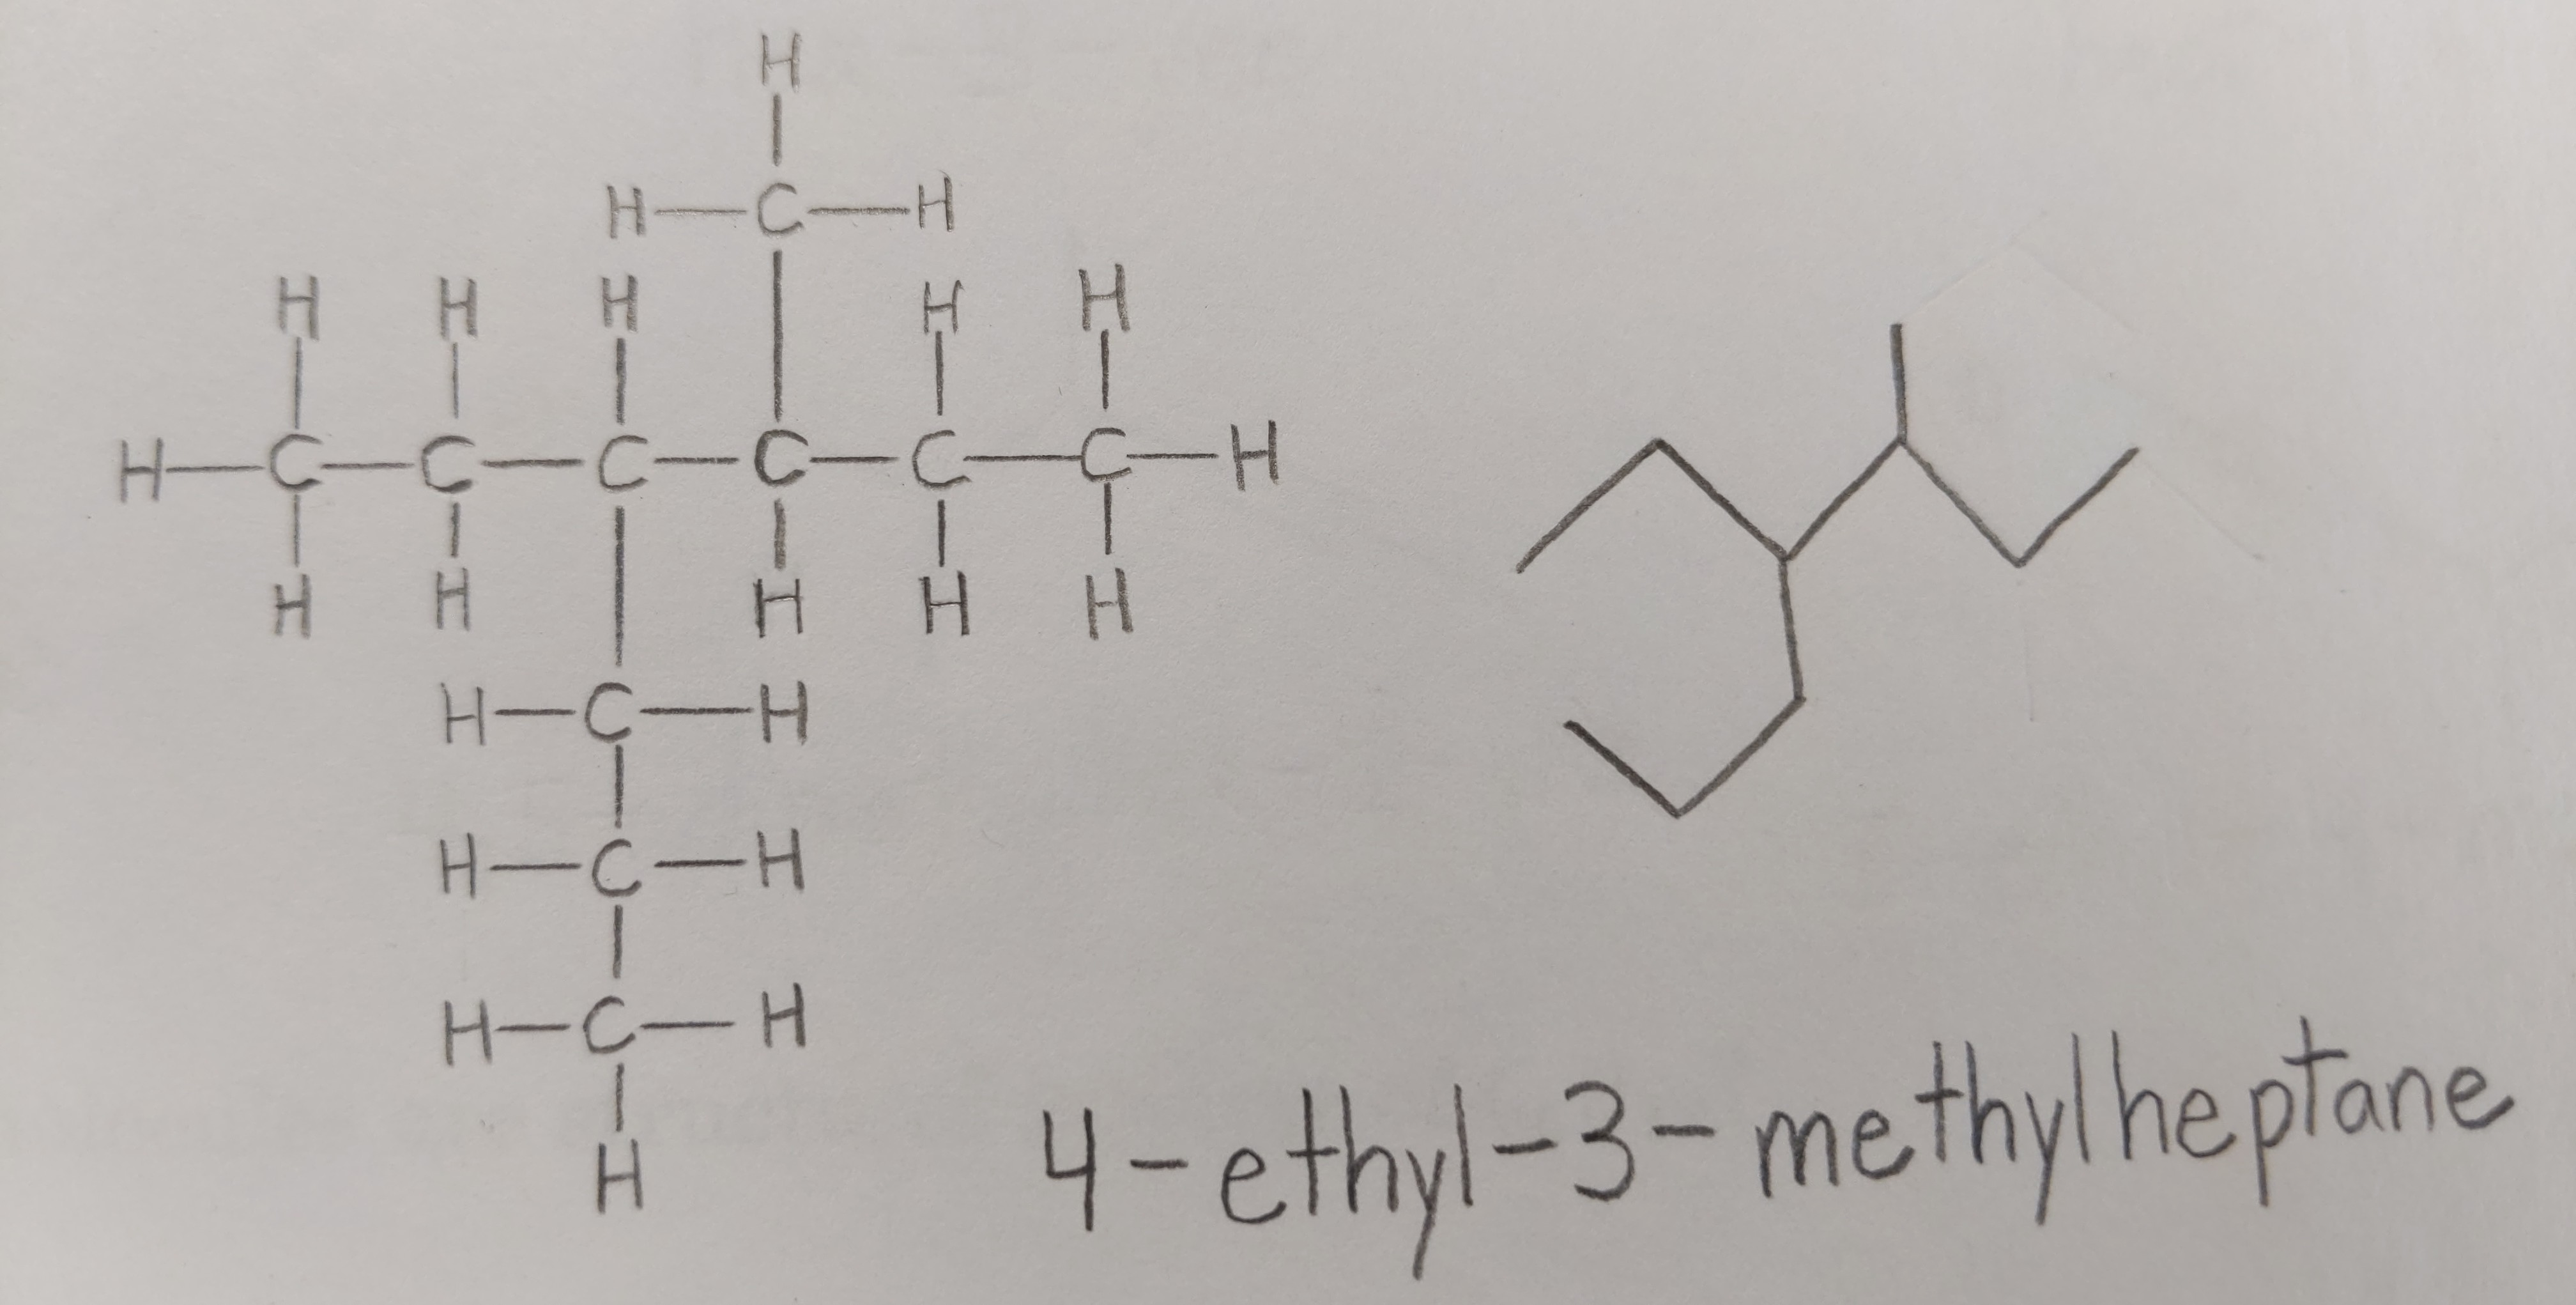
\includegraphics[scale=0.053]{diagrams/organic-molecule.jpg}
        \label{fig:organic}
    \end{figure}
    \end{enumerate}
    \end{minipage}
};
%------------ Drawing Organic Molecules ---------------------
\node[fancytitle, right=10pt] at (box.north west) {Drawing Organic Molecules};
\end{tikzpicture}

%------------ Hydrocarbons ---------------
\begin{tikzpicture}
\node [mybox] (box){%
    \begin{minipage}{0.3\textwidth}
    \small{
    \begin{tikzpicture}[level distance=1.3cm,
        level 1/.style={sibling distance=4cm},
	level 2/.style={sibling distance=1.5cm}]
	\centering
	\node {Hydrocarbons}
	    child {node {Aliphatic}
	    child {node {Alkanes}}
	    child {node {Alkenes}}
	    child {node {Alkynes}}
	    }
	    child {node {Aromatic}
	    child {node {Aromatic}}
	    };
    \end{tikzpicture}} \\
    \textbf{Hydrocarbon}: compound that contains only carbon atoms and hydrogen atoms. \\
    $\rightarrow$ The simplest hydrocarbons are \textit{alkanes}. \\
    \textbf{Aromatic Hydrocarbon}: compound containing only carbon and hydrogen and based on the aromatic benzene. \\
    \textbf{Hückel's Rule}: aromatic compounds contain $4n+2\,\pi\,e^{-}$. \\
    \textbf{Cyclic Hydrocarbon}: an aliphatic hydrocarbon chain that forms a ring (but not a benzene ring). \\
    \textbf{Saturated Hydrocarbon}: organic compound that contains only single bonds, with no double or triple bonds between carbon atoms. e.g. alkanes. \\
    \textbf{Unsaturated Hydrocarbon}: hydrocarbon that contains carbon-carbon double or triple bonds, whose carbon atoms can bond to additional atoms. e.g. alkenes, alkynes. \\
    \textbf{Isomers}: molecules that have the same molecular formula but their atoms are in a different arrangement. \\
    \textbf{Structural Isomers}: molecules that have the same molecular formula but their atoms are bonded together in a different sequence. \\
    e.g. pentane is a structural isomer of $C_{5}H_{12}$. \\
    \textbf{Stereoisomers}: molecules that have the same molecular formula and their atoms are bonded together in the same sequence, but differ in the three-dimensional orientations of their atoms in space.
    \begin{itemize}
        \item \textit{trans} isomer - two identical atoms or groups are on the opposite sides of the double bond
        \item \textit{cis} isomer - two identical atoms or groups are on the same side of the double bond
    \end{itemize}
    \textbf{Diastereomers}: a stereoisomer based on a double bond.
    \textbf{Enantiomer}: a stereoisomer in which molecules are mirror images of each other around a single carbon atom bonded to four different types of atoms or groups. \\
    \textbf{Primary, Secondary, and Tertiary}:
    \begin{itemize}
        \item primary (terminal) carbon is labelled with an ``n-''
	\item secondary carbon is labelled with an ``s-'' or ``sec-''
	\item tertiary carbon is labelled with a ``t-'' or ``tert-''
    \end{itemize}
    \end{minipage}
};
%------------ Hydrocarbons Header ---------------------
\node[fancytitle, right=10pt] at (box.north west) {Hydrocarbons};
\end{tikzpicture}

%------------ Nomenclature ---------------
\begin{tikzpicture}
\node [mybox] (box){%
    \begin{minipage}{0.3\textwidth}
    The \textbf{root} denotes the number of carbon atoms in the longest continuous chain of carbon atoms. \\
    The \textbf{prefix} gives the positions and names of any branches from the main chain. \\
    The \textbf{suffix} indicates the series to which the molecule belongs (e.g., the suffix for alkanes is ``-ane'').
    \begin{enumerate}
        \item highest priority group is used as the main name
	\item the molecule is numbered to give the highest priority group the smallest numbers
        \item all other groups are listed alphabetically
    \end{enumerate}
    \begin{tabular}{| c | c | c |}
        \hline
	Number of & & Side Group \\
	Carbon Atoms & Root Name & Name \\ \hline
        1 & meth- & methyl- \\ \hline
        2 & eth- & ethyl- \\ \hline
        3 & prop- & propyl- \\ \hline
        4 & but- & butyl- \\ \hline
        5 & pent- & pentyl- \\ \hline
        6 & hex- & hexyl- \\ \hline
        7 & hept- & \\ \hline
        8 & oct- & \\ \hline
        9 & non- & \\ \hline
        10 & dec- & \\ \hline
    \end{tabular} \\ \\
    \textbf{Functional Group Priority List}:
    \begin{enumerate}
        \item Carboxylic Acid $\rightarrow$ ``-oic acid''
	\item Ester $\rightarrow$ ``-oate''
	\item Amide $\rightarrow$ ``-amide''
	\item Aldehyde $\rightarrow$ ``-al''
	\item Ketone $\rightarrow$ ``-one''
	\item Alcohol $\rightarrow$ ``-ol'', ``hydroxy-'' as substituent
	\item Amine $\rightarrow$ ``-amine'', ``amino-'' as substituent
	\item Alkene/Alkyne $\rightarrow$ ``-ene'' has priority over ``-yne''
	\item Alkane $\rightarrow$ ``-ane''
	\item Ether/Alkyl Halide/Nitro $\rightarrow$ ``alkoxy-''/``iodo-'', ``fluoro-'', ``chloro-'', and ``bromo-''/``nitro-''
    \end{enumerate}
    \end{minipage}
};
%------------ Nomenclature Header ---------------------
\node[fancytitle, right=10pt] at (box.north west) {Nomenclature};
\end{tikzpicture}

%------------ Functional Groups ---------------
\begin{tikzpicture}
\node [mybox] (box){%
    \begin{minipage}{0.3\textwidth}
    \textbf{Substituent Group}: atom or group of atoms substituted in place of a hydrogen atom on the parent chain of an organic compound. \\
    \textbf{Functional Group}: a special arrangement of atoms that is mainly responsible for the chemical behaviour of the molecule. \\
    \textbf{Alkane}: a hydrocarbon molecule in which the carbon atoms are joined by single covalent bonds. \\
    $\hookrightarrow$ Soluble in benzene and other non-polar solvents. \\
    \textbf{Alkene}: a hydrocarbon molecule that contains one or more carbon-carbon double bonds. \\
    $\hookrightarrow$ Location of double bond affects boiling point. \\
    \textbf{Alkyne}: a hydrocarbon molecule that contains one or more carbon-carbon triple bonds. \\
    $\hookrightarrow$ Alkynes are always linear around the triple bond. \\
    \textbf{Alkyl Group}: a side group based on an alkane. \\
    e.g. the \ce{-CH_3} group is called a methyl group. \\
    \textbf{Phenyl Group}: term used for a benzene ring that forms a substituent group on a hydrocarbon chain. \\
    \textbf{Alcohol}: a hydrocarbon derivative that contains a hydroxyl group. \\
    \textbf{Hydroxyl Group}: consists of an oxygen atom and a hydrogen atom (\ce{-OH}). \\
    \textbf{Haloalkane}: a hydrocarbon derivative that contains at least one halogen atom. \\
    \textbf{Carbonyl Group}: consists of a carbon atom that is double bonded to an oxygen atom (\ce{$>$C=O}). \\
    \textbf{Aldehyde}: a hydrocarbon derivative that contains a carbonyl group that is on the terminal carbon. \\
    \textbf{Ketone}: a hydrocarbon derivative that contains a carbonyl group that is on the secondary carbon; it is bonded to two carbon atoms or carbon chains. \\
    \textbf{Carboxylic Acid}: a hydrocarbon derivative that contains a carboxyl group. \\
    \textbf{Carboxyl Group}: consists of a carbonyl group with a hydroxyl group attached to it (\ce{-COOH}).
    \begin{figure}[H]
        \centering
        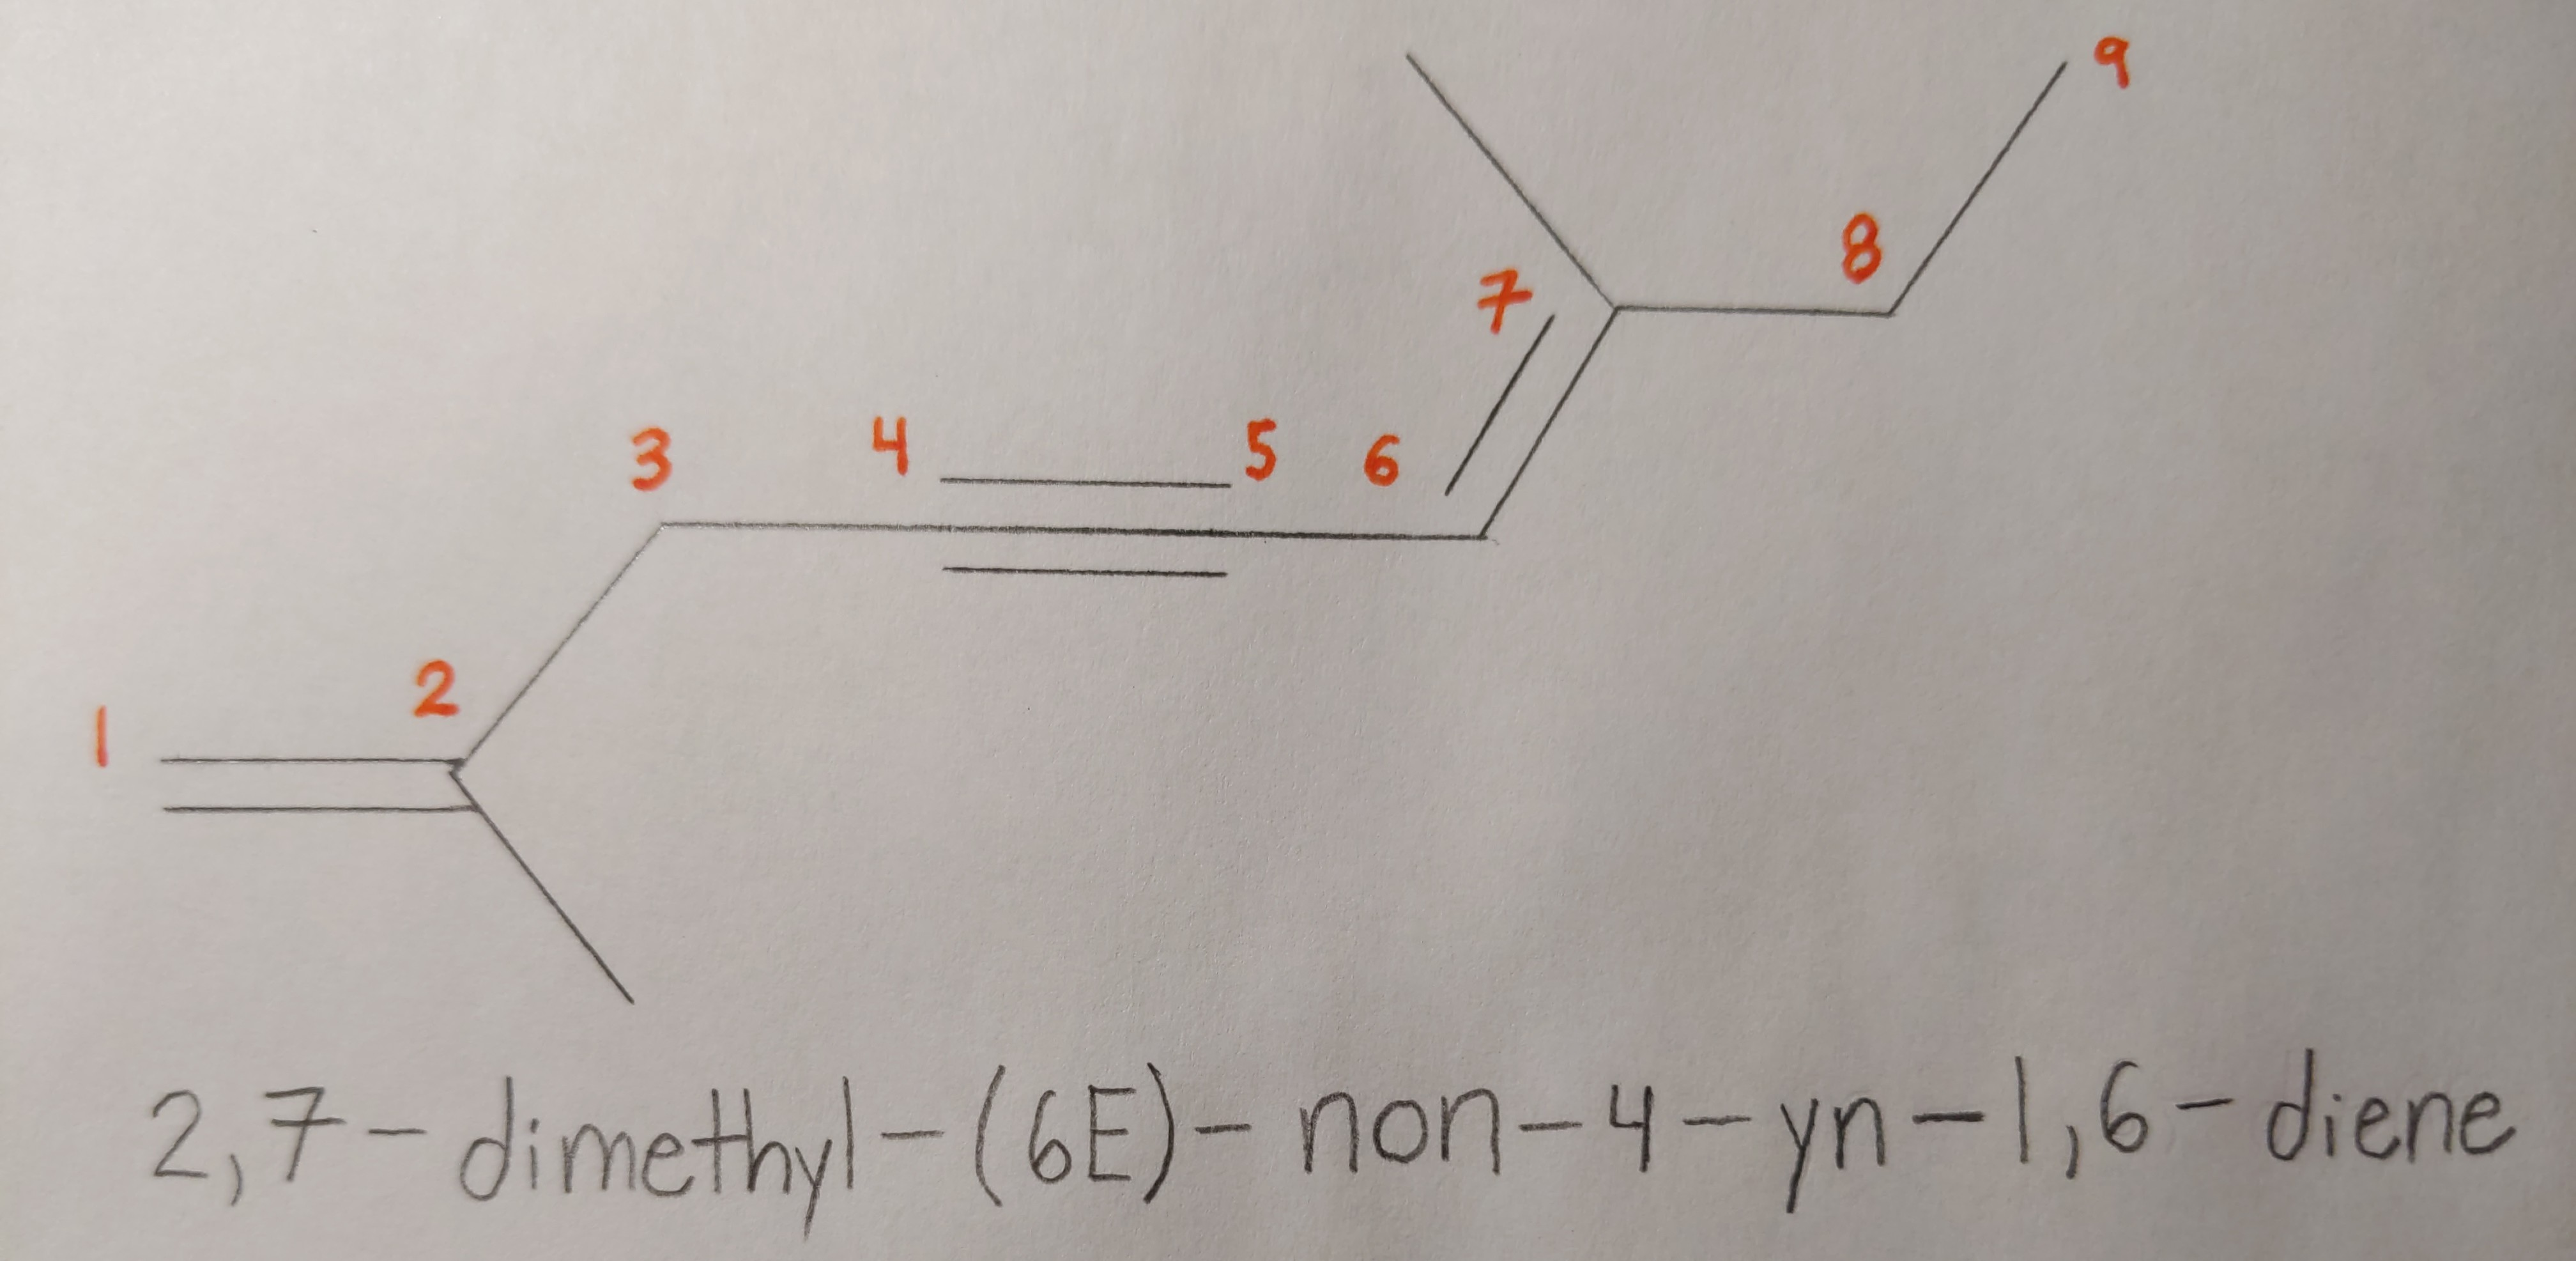
\includegraphics[scale=0.054]{diagrams/naming-rules.jpg}
        \label{fig:naming}
    \end{figure}
    \end{minipage}
};
%------------ Functional Groups Header ---------------------
\node[fancytitle, right=10pt] at (box.north west) {Functional Groups};
\end{tikzpicture}

%------------ Functional Groups Continued ---------------
\begin{tikzpicture}
\node [mybox] (box){%
    \begin{minipage}{0.3\textwidth}
    \textbf{Ester}: a hydrocarbon derivative that contains a functional group with a carbon atom double bonded to one oxygen atom and single bonded to another (\ce{RCOOR$'$}). \\
    \textbf{Ether}: a hydrocarbon derivative in which an oxygen atom is single bonded to two carbon atoms (\ce{R-O-R$'$}). \\
    \textbf{Alkoxy Group}: a side group found in an ether that includes the oxygen atom and the shorter alkyl group bonded to it (\ce{-O-}). \\
    \textbf{Amine}: a hydrocarbon derivative that contains a nitrogen atom bonded to at least one carbon atom, although it may be bonded to up to three. \\
    \textbf{Amide}: a hydrocarbon derivative that contains a carbonyl group bonded to a nitrogen atom (\ce{-CON-}).
    \end{minipage}
};
%------------ Functional Groups Continued Header ---------------------
\node[fancytitle, right=10pt] at (box.north west) {Functional Groups Continued};
\end{tikzpicture}

%------------ Addition Reactions ---------------
\begin{tikzpicture}
\node [mybox] (box){%
    \begin{minipage}{0.3\textwidth}
    \textbf{Addition Reaction}: reaction in which atoms are added to a carbon-carbon double or triple bond. \\
    \textbf{Markovnikov's Rule}: hydrogen atom of the small molecule will attach to the carbon of the double bond that is already bonded to the most hydrogen atoms. \\
    \textbf{Electrophile}: accepts an electron pair (Lewis acid). \\
    \textbf{Nucleophile}: donates an electron pair (Lewis base).
    \begin{itemize}
	\item check whether the carbon atoms in the product(s) are bonded to \textit{more} atoms than are the carbon atoms in the organic reactant
	\item the groups added can be: halogen (halogenation), hydrogen (hydrogenation), water (hydration), hydrogen + halogen (hydrohalogenation)
    \end{itemize}
    \end{minipage}
};
%------------ Addition Reactions Header ---------------------
\node[fancytitle, right=10pt] at (box.north west) {Addition Reactions};
\end{tikzpicture}

%------------ Elimination Reactions ---------------
\begin{tikzpicture}
\node [mybox] (box){%
    \begin{minipage}{0.3\textwidth}
    \textbf{Elimination Reaction}: atoms are removed from an organic molecule to form a double bond. (\ce{->[\Delta]})
    \begin{itemize}
	\item determine whether the carbon atoms in the organic product are bonded to fewer atoms than were the carbon atoms in the organic reactant
	\item as a general rule, the hydrogen atom is most likely to be removed from the carbon atom with the most carbon-carbon bonds
	\item must have an electronegative group and a base must be present in solution to remove a proton
    \end{itemize}
    \end{minipage}
};
%------------ Elimination Reactions Header ---------------------
\node[fancytitle, right=10pt] at (box.north west) {Elimination Reactions};
\end{tikzpicture}

%------------ Substitution Reactions ---------------
\begin{tikzpicture}
\node [mybox] (box){%
    \begin{minipage}{0.3\textwidth}
    \textbf{Substitution Reaction}: reaction in which a hydrogen atom or functional group is replaced by a different atom or functional group.
    \begin{itemize}
        \item \textit{two} compounds react to form two different compounds
        \item \textit{carbon} atoms are bonded to the \textit{same} number of atoms in the product as in the reactant
	\item results in the creation of amines, alcohols, ethers, and alkyl halides (require UV light)
    \end{itemize}
    \end{minipage}
};
%------------ Substitution Reactions Header ---------------------
\node[fancytitle, right=10pt] at (box.north west) {Substitution Reactions};
\end{tikzpicture}

%------------ Condensation Reactions ---------------
\begin{tikzpicture}
\node [mybox] (box){%
    \begin{minipage}{0.3\textwidth}
    \textbf{Condensation Reaction}: two large molecules combine to form one larger molecule and a very small molecule, usually water. \\
    \textbf{Esterification Reaction}: a special type of condensation reaction.
    \begin{itemize}
        \item \ce{carboxylic acid + amine -> amide + water}
        \item \ce{alcohol + alcohol -> ether + water}
        \item \ce{alcohol + carboxylic acid -> ester + water}
    \end{itemize}
    \end{minipage}
};
%------------ Condensation Reactions Header ---------------------
\node[fancytitle, right=10pt] at (box.north west) {Condensation Reactions};
\end{tikzpicture}

%------------ Hydrolysis Reactions ---------------
\begin{tikzpicture}
\node [mybox] (box){%
    \begin{minipage}{0.3\textwidth}
    \textbf{Hydrolysis Reaction}: a molecule is broken apart by adding the hydroxyl group from a water molecule to one side of a bond and the hydrogen atom of a water molecule to the other side of the bond. \\
    $\star$ Both the condensation reaction and the hydrolysis reaction are catalyzed by an acid (they are reversible).
    \end{minipage}
};
%------------ Hydrolysis Reactions Header ---------------------
\node[fancytitle, right=10pt] at (box.north west) {Hydrolysis Reactions};
\end{tikzpicture}

%------------ Polymers ---------------
\begin{tikzpicture}
\node [mybox] (box){%
    \begin{minipage}{0.3\textwidth}
    \textbf{Polymer}: a large, long-chain molecule with repeating units of small molecules called monomers. \\
    e.g. \ce{sodium tetraborate (borax) + vinyl acetate (glue)} \\
    \textbf{Monomer}: small molecule, linked covalently to others of the same or similar type to form a polymer. \\
    \textbf{Addition Polymerization}: reaction in which alkene monomers are joined through multiple addition reactions to form a polymer. \\
    \textbf{Condensation Polymerization}: reaction in which monomers are combined through multiple condensation reactions to form a polymer. \\
    $\star$ Formation of ester or amide linkages in the product.
    \end{minipage}
};
%------------ Polymers Header ---------------------
\node[fancytitle, right=10pt] at (box.north west) {Polymers};
\end{tikzpicture}

\end{multicols*}
\end{document}
